%----------------------------------------------------------------------------------------
%   PACKAGES AND OTHER DOCUMENT CONFIGURATIONS
%----------------------------------------------------------------------------------------

% latexmk -pvc -pdf
\documentclass[12pt, a4paper, openany]{book}
\usepackage[margin=2.5cm]{geometry}
\usepackage{titling}
\usepackage{titlesec}
\usepackage{amsmath,amsthm,amsfonts,amssymb}
\usepackage{dsfont}
\usepackage{mathtools}
\usepackage{braket}
\usepackage[font=scriptsize,labelfont=bf]{caption}
\usepackage[english]{babel}

\usepackage{cite}

\usepackage{datetime}
\newdateformat{monthyeardate}{%
  \monthname[\THEMONTH], \THEYEAR}

\usepackage{graphicx}
\newenvironment{Figure}
    {\par\medskip\noindent\minipage{\linewidth}}
    {\endminipage\par\medskip}
\usepackage{tabularx}

\newenvironment{abstract}
{\clearpage \thispagestyle{empty} \null \vfill \begin{center} \bfseries \large Abstract \end{center}}
{\vfill \null \clearpage}

% Colours:
\usepackage[table]{xcolor} % for setting colors
\definecolor{purple}{RGB}{117,77,226}

\usepackage[bookmarksopen,
  pagebackref,
  pdfpagelayout=TwoPageRight,
  colorlinks=true,
  urlcolor=purple,
  citecolor=purple,
  filecolor=purple,
  linkcolor=purple,
  ]
{hyperref}

\usepackage{listings}
\usepackage{xcolor} % Necessary to define custom colors

\definecolor{softblue}{rgb}{0.3, 0.5, 0.8}
\definecolor{darkergreen}{rgb}{0, 0.5, 0}

\lstset{
  basicstyle=\ttfamily\small, % Set the typeface to typewriter and small size
  breaklines=true, % Enable line breaking
  postbreak=\mbox{\textcolor{red}{$\hookrightarrow$}\space}, % Marker for line breaks
  numbers=left, % Line numbers on left
  numberstyle=\tiny, % Set the size of the numbers
}

% \lstset{
%     literate=%
%     {ö}{{\"o}}1
%     {Ψ}{{$\Psi$}}1
%     {Φ}{{$\Phi$}}1
% }

\lstdefinestyle{mystyleC}{
    language=C,      
    commentstyle=\color{softblue},
    morecomment=[l]{//},  % Line comment
}

\lstdefinestyle{mystylePython}{
    language=Python,      
    commentstyle=\color{darkergreen},
    morecomment=[l]{//},  % Line comment
}

\titleformat{\chapter}[display]
  {\normalfont\bfseries}{}{0pt}{\Huge}

\newcommand\II{\(\mathcal{I}\)}
\newcommand\PT{\(\mathcal{PT}\)}
\newcommand\PP{\(\mathcal{P}\)}
\newcommand\TT{\(\mathcal{T}\)}
\newcommand\CPT{\(\mathcal{CPT}\)}
\newcommand\CC{\(\mathcal{C}\)}


% Required packages
\usepackage{catchfile}

% Command to execute texcount and capture the word count
\newcommand\wordcount[1]{
    \immediate\write18{texcount #1.tex | grep "Words in text" | cut -d: -f2 > #1.wordcount.tmp}
    \CatchFileDef{\mywordcount}{#1.wordcount.tmp}{}
    \immediate\write18{rm #1.wordcount.tmp} % to remove the temporary file
    \mywordcount % to print the word count
}


\begin{document}

\begin{titlepage}
\begin{center}
    {\Huge BEDSAT:Antarctica}\\ [1cm] 
    {\Large random writings}\\ [2cm]
    {\large Ana Fabela Hinojosa\footnote{ana.fabelah@gmail.com}}\\ [1cm]
    Supervisors:\\
    Dr. Felicity McCormack\\
    Dr Jason Roberts\\
    Dr Richard Jones\\ [2cm]


    
\includegraphics[scale=0.3]{logo.jpg}\\ [-0.7cm]
    \textsc{School of Earth, Atmosphere and Environment}\\ [1cm]
    \monthyeardate\today
\end{center}
\end{titlepage}


%----------------------------------------------------------------------------------------
%   QUOTATION PAGE
%----------------------------------------------------------------------------------------
% \vspace*{0.2\textheight}

% \noindent{``El alacrán clavándose el aguijón, harto de ser un alacrán pero necesitando de su alacranidad para acabar con el alacrán''.}\bigbreak
% % \vspace{-2cm}
% \hfill Julio Cortázar\bigbreak

\begin{abstract}\label{abstracc}
Antarctica has been losing ice mass over recent decades, contributing to rising sea levels, but there is significant uncertainty regarding the extent and timing of this ice loss due to unknown ice sheet properties and flow processes. One key factor influencing ice flow and loss is bed topography, typically derived from sparse airborne radar surveys with high uncertainties. These uncertainties impact simulations of the Antarctic Ice Sheet (AIS) evolution under climate change. Given the logistical challenges of surveying Antarctica, alternative approaches, including satellite data integration, are needed. Two common methods for estimating bed topography are the mass conservation (MC) method and geostatistics. The MC method uses satellite-derived surface velocity estimates and physical laws of mass and momentum conservation to calculate ice thickness and bed topography, but it is limited to regions where ice flow exceeds 50 meters per year, mostly near the coast. Its accuracy depends on the spacing of ice thickness measurements and uncertainties in ice velocity and surface mass balance. Geostatistical methods refine bed topography resolution using radar-derived measurements, but like MC, they are more effective near the coast. These methods have advanced our understanding of glacier dynamics and other processes but face limitations, especially in the continent's interior. This project proposes a new method, BedSAT, which leverages the mathematical relationship between ice surface elevation and bed topography to estimate bed topography using high-resolution ice surface elevation data, enhancing ice sheet models and reducing uncertainties in bed topography estimates.
\end{abstract}

% \chapter*{Acknowledgements}

% \tableofcontents

\chapter{An example of previous work modelling the bedrock topography}\label{n1}

Numerical modelling, sedimentary sequence interpretation suggest cyclical periods of ice-sheet expansion and retreat\cite{Young2011}. Using ice-penetrating radar data to generate a new basal bed topography of the Aurora Subglacial Basin (ASB) in east Antarctica is characterised by a fjord landscape (this land is under $\sim$ under $2-4.5$ km of ice). The ASB has a potentially significant influence on the east Antarctic ice-sheet (EAIS), however there is high uncertainty in estimates of past and present global sea level changes due to the scarcity of bed data\cite{Young2011}. This uncertainty also limits the accuracy of models used to predict future ice sheet growth or decay.\\

{\large Methods in\cite{Young2011}}
\begin{enumerate}
    \item A ski-equipped airplane (DC-3T) carried a radar system (HiCARS), which can see through ice. HiCARS sends signals that bounce back to show the thickness of the ice and the shape of the land beneath it.
    \item The plane flew back and forth over a large area, covering distances of around 1,000 km. The flights took place over two different periods in 2008–2009 and 2009–2010.
    \item The radar data was cleaned up (processed) to improve accuracy, and they used a special radar system that helps reduce distortions (errors) in the measurements. \textbf{[HOW?]}
    \item Thickness of the ice was measured using the time it took for the radar signals to travel through the ice and back, assuming the radar signals move through the ice at a specific speed (169 meters per microsecond).
    \item The height of the land below the ice was calculated by looking at the radar-determined surface of the ice. \textbf{[WHAT?]}
    \item The radar data was combined with other existing datasets (BEDMAP) to improve the overall picture. They used a computer algorithm to fill in gaps where they didn’t have direct measurements. \textbf{[WHICH?]}
    \item Determining how rough or uneven the land under the ice was, by using a statistical measure called the ''root mean squared (rms) deviation."
\end{enumerate}

In short, Young et al. used advanced radar technology on an airplane to map the ice thickness and the landscape beneath it in a region of Antarctica, combining this data with previous maps for a better overall picture.

\chapter{IPCC Special Report 2019}\label{n2}
\textbf{WHY IS IMPORTANT TO DEVELOP BETTER TOPOGRAPHIC MODELS OF THE ANTARCTIC CONTINENT?}
The polar regions are losing ice, and their oceans are changing rapidly. The consequences of this polar transition extend to the whole planet and it is crucial for us to understand them and plan for changes.
\begin{itemize}
\item Climate-induced changes in seasonal ice extent and thickness are affecting sea ice and ocean layers, which impacts marine plant growth (highly likely). This alters ecosystems (moderately likely). The timing and amount of plant growth have changed in both polar oceans, varying by location (highly likely). In Antarctica, these changes relate to retreating glaciers and sea ice change (moderately likely). In the Arctic, they've affected the types, locations, and numbers of marine species, changing ecosystem structure (moderately likely)\cite{O_C_in_changingClimate}.
\item The rapid ice loss from the Greenland and Antarctic ice sheets during the early 21st century has increased into the near present day, adding to the ice sheet contribution to global sea level rise (extremely likely)\cite{O_C_in_changingClimate}.
\item Both polar oceans will be increasingly affected by $\mathrm{CO_2}$ uptake, causing conditions corrosive for calcium carbonate shell-producing organisms (high confidence), with associated impacts on marine organisms and ecosystems (medium confidence)\cite{O_C_in_changingClimate}.
\item change in thermohaline circulation....
\end{itemize}

Temperature changes in Antarctica:
Unlike the Arctic, which has seen uniform warming, Antarctica's temperature changes have been less consistent. West Antarctica has warmed in some parts. East Antarctica hasn't shown significant overall change. in the past 3-5 decades. There's low confidence in these observations due to limited data and high variability.

Why Antarctica isn't warming as much as the Arctic:
The Southern Ocean surrounding Antarctica absorbs and mixes heat deep into the ocean\cite{L_T_C_C}.


Factors influencing Antarctic climate:

Three main atmospheric patterns affect Antarctica's climate and sea ice:
a) Southern Annular Mode (SAM)
b) Pacific South American mode
c) Zonal-wave 3


Recent changes in the Southern Annular Mode (SAM):

The SAM has been mostly positive in recent decades during summer.
This means stronger westerly winds around Antarctica.
This positive phase is unprecedented in at least 600 years.
It's associated with cooler conditions over Antarctica.


Causes of SAM changes:

Ozone depletion was likely the main driver of SAM changes from the late 1970s to late 1990s.
Since 2000, tropical sea surface temperatures have played a stronger role in influencing SAM.


Other influences on Antarctic climate:

Tropical sea surface temperatures can affect Antarctic temperatures and Southern Hemisphere mid-latitude circulation\cite{JACOBS_2004}.



In summary, Antarctica's climate is complex and influenced by various factors, with recent changes differing from those in the Arctic due to unique ocean and atmospheric patterns.

\begin{Figure}
\centering
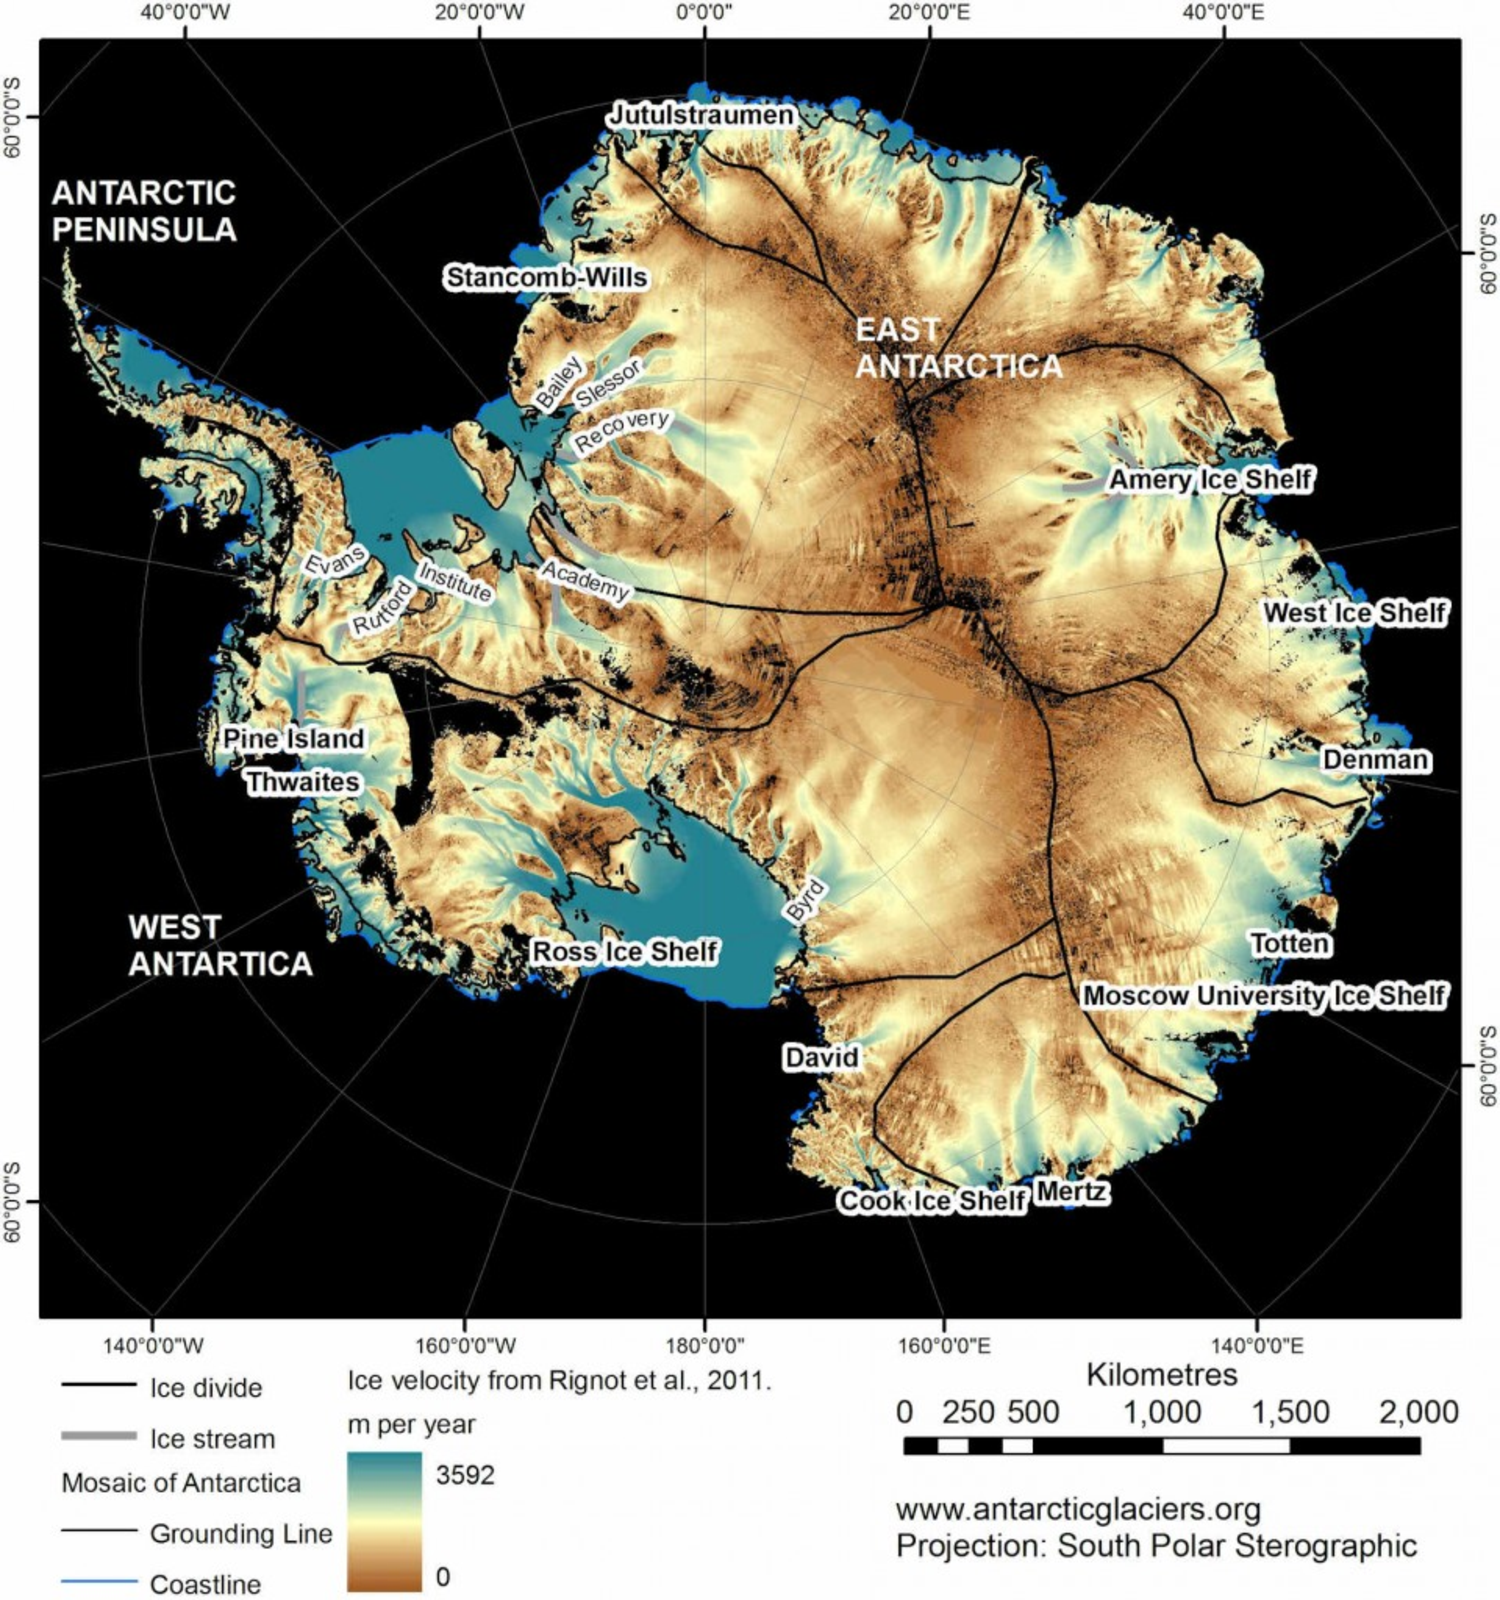
\includegraphics[width=1.1\linewidth]{antarctica_velocity.pdf}
\captionof{figure}{}
\label{fig:Antarctica_velocity}
\end{Figure}

Unknown terms
{\small \begin{itemize}
\item{Channel incision}
\item{Alpine style glaciation}
\end{itemize}
}
\vspace{1cm}
TOOLS
{\small \begin{itemize}
\item{ICECAP aero geophysical programme}
\item{BEDMAP}
\end{itemize}
}
\vspace{1cm}
MATHS
{\small \begin{itemize}
\item{Lagrangian interpolation}
\item{natural-neighbour interpolation}
\end{itemize}
}


\wordcount{notes1} words in this section.
% %
% \include{complexandcomplicated}
% % \wordcount{complexandcomplicated} words in this section.
% % 
% \include{dynamics}
% % \wordcount{dynamics} words in this section.
% %
% \include{Conclusion}
% % \wordcount{Conclusion} words in this section.
% %
% \appendix
% \include{appendix}
% % \wordcount{appendix} words in this section.

\bibliographystyle{unsrturl_mod}
\bibliography{mybib}
\end{document}


